%% Semplice beamer conforme al powerpoint ufficiale
%% dal sito di Ca' Foscari. Si basa sul tema "default"
%% mandate Modifiche e migliorie! Guido.Caldarelli@unive.it 
% Elenco Contributori 
% Guido Caldarelli, Matteo Brilli 

%\documentclass{beamer}
% decide below the aspect ratio between 16:9 and 4:3
%\documentclass[aspectratio=43]{beamer}
\documentclass[aspectratio=169]{beamer}

\usepackage[utf8]{inputenc}
\usepackage{booktabs}
\usepackage{csquotes}
\usepackage[style=authoryear,backend=biber]{biblatex}
\addbibresource{bibliography/intro-ch-02-culturonomics.bib}

\addtolength{\skip\footins}{4pc plus 8pt}

% Questo tema commentato di sotto produce un beamer più tradizionale 
%\usetheme[secheader]{Boadilla}


%%%-----------------------------------------------------------%
%% Cambia colori da thema default
%% Questi sono i due colori ufficiali rosso e grigio
\definecolor {cfred}{rgb}{0.709,0.196,0.329} 	%{ 181 ,50 ,84}
\definecolor {cfgrey}{rgb}{0.537,0.537,0.537} 	%{ 137,137,137}
\definecolor {cflink}{rgb}{0.615,0.615,0.607} 	%{157,157,155}

\setbeamercolor{palette primary}{bg=cfred,fg=white}
\setbeamercolor{palette secondary}{bg=cfred,fg=white}
\setbeamercolor{palette tertiary}{bg=cfred,fg=white}
\setbeamercolor{palette quaternary}{bg=cfred,fg=white}
\setbeamercolor{structure}{fg=cfred}		 % itemize, enumerate, etc
\setbeamercolor{section in toc}{fg=cfred} 		 % TOC sections
% Override palette coloring with secondary
\setbeamercolor{subsection in head/foot}{bg=cfgrey,fg=white}
%%%------------------------------------------------------------

%% Definisce il blocco con riquadro che non è presente nel tema default (commentare se si usano altri temi)
\setbeamercolor{uppercolor}{fg=white,bg=cfred}%
\setbeamercolor{lowercolor}{fg=black,bg=white}%
\def \bblock{\begin{beamerboxesrounded}[upper=uppercolor,lower=lowercolor,shadow=true]}
\def \eblock{\end{beamerboxesrounded}}

\defbeamertemplate{description item}{align left}{\insertdescriptionitem\hfill}
\setbeamertemplate{description item}[align left]
%%-----------------------------------------------------------

%% Intestazione ripetuta per ogni slide
\addtobeamertemplate{headline}{%
    \vspace{0.25cm} \ \ 
    
\includegraphics[height=1.0cm]{images/fedhlab4.png} 	% sostituire con logobeamIT.png per italiano
    \hspace{0.541\textwidth}{\color{cflink} {\small Intro. to CH}} %per 16:9 641 for link
    %\hspace{0.551\textwidth}{\color{cflink} {\small www.unive.it}} %per 4::3
    \vspace{0.25cm}
    {\color{cfred} \hrule \hrule  }
    \textbf{}
}{}
\setbeamertemplate{footline}[text line]{%
  \parbox{\linewidth}{\vspace*{-8pt}%
  {\color{cflink} {%
  Page \insertpagenumber/\inserttotalframenumber~--  CC-BY-NC 4.0 -- thibault.clerice@inria.fr
}}}}

\setbeamertemplate{page number in head/foot}[appendixframenumber]
%%-------------------------------------------------------------

%This block of code defines the information to appear in the Title page
%%%
\title[Intro to CH] %optional
{From Digital Humanities to Computational Humanities}\subtitle{The Example of Latin Digital Philology}

\author[Clérice, Thibault] % (optional)
{T.~Clérice~\inst{1}~\inst{2}}

\institute[Inria] % (optional)
{
  \inst{1}%
  ALMAnaCH, Inria, Paris, France \and
  \inst{2}%
  FeDHLab, Università Federico II, Napoli, Italia
 }

\date[2024] % (optional)
{Introduction to Computational Humanities}

\setbeamertemplate{frametitle}[default][right, rightskip=.5cm] {}
\addtobeamertemplate{frametitle}{\vspace*{-1.4cm}}{}
%End of title page configuration block
%------------------------------------------------------------


%------------------------------------------------------------
%The next block of commands puts the table of contents at the 
%beginning of each section and highlights the current section:

\AtBeginSection[]
{
  \begin{frame}
    \frametitle{Table of Contents}
    \tableofcontents[currentsection]
  \end{frame}
}
%------------------------------------------------------------

\setbeamerfont{footnote}{size=\tiny} %reduce the size of the footnote citation

\addtobeamertemplate{footnote}{}{\vspace{2.2ex}}
\begin{document}

%The next statement creates the title page.
\frame{\titlepage}


\section{Introduction}

\begin{frame}{Culturonomics, corpus linguistics, what changed ?}
    \fullcite{brunet:hal-01362715}
    \begin{itemize}
        \item Textual Statistics/Frequencies $\rightarrow$ Lexicometry $\rightarrow$ Culturonomics ?
        \item Statistics in texts is "old", studies into Plato frequencies regarding its style starts in the 1870s\footfullcite{plato}.
        \item Zipf's law $\approx$ 1940s": most frequent word appears two times more than next most frequent one.
    \end{itemize}
\end{frame}

% \begin{frame}{Frame Title}
    
% \end{frame}

\begin{frame}{Today's papers}

    \begin{itemize}
        \item \fullcite{michel2011quantitative}
        \item \fullcite{camps2023make}
        \item \fullcite{denove2024industrial}
        \item \fullcite{perreaux:halshs-01148891}
    \end{itemize}
    
\end{frame}

\begin{frame}{Culturonomics}
    
\end{frame}

\section{Funding Paper of Culturonomics}

\begin{frame}{A first comment}
    \begin{itemize}
        \item In the author list, none of the writers identifies as a member of a Linguistic department.
        \item The abstract, in a computer science and a GAFAM fashion, promises a revolution spanning the social sciences and the humanities. Except that only Michel is connected to Cultural or humanities studies, and even more so apparently from the Psychology and evolutionary side of things.
        \item While I would have the same bias, and at least it provides for a baseline, the paper only approaches culture through printed documents: it ignores not only private literature (postcards, letters, etc.), but also paintings, radio recordings, and more importantly over the last decades, movies and TV-related outputs.
    \end{itemize}
\end{frame}

\begin{frame}{A new (dirty ?) corpus }
    \begin{itemize}
        \item Statistically sound: 4\% of all the printed books makes for a representative sample
        \item Header, page number and footer are identified for cleaning noise (Online, Supplementary Material, I.3) 
        \item But is it representative ?
        \begin{itemize}
            \item No smoothing of the sampling: more texts are taken in the 1950-2000 section than in the 1900-2000
            \item Periodical excluded (without any discussions ???)
        \end{itemize}
        \item and is it clean ?
        \begin{itemize}
            \item In the supplementary material, it is clear that some machine learning machine was used to deduplicate texts from a metadata point of view, but not from a content point of view.
        \end{itemize}
    \end{itemize}
\end{frame}

\begin{frame}{5 experiments for Culturomics}
    Discussion time
    \begin{itemize}
        \item The Lexicon ``Challenge'' \note{Here, the bias of the corpus (mostly literary in 1800, more and more technical after,) is probably important. Plus, is it really the role of a dictionary/lexicon to register ALL the words that exist ? And what of the method to define what is a word ?}
        \item The ``Evolution'' of Grammar \note{Only really a history of morphology, and the bias in the corpus might hide a very important fact regarding the normalization of certain form.}
        \item Memorization \note{Maybe the best argument, but it also ignores the fact that classics or important books are reprinted. So what is the value of a reprinted word ? Does it reactualize the memory of something or someone ? Do we need new books on Cicero every year to remember him ?}
        \item Fame duration \note{Again, books reprint}
        \item Censorship \note{}
    \end{itemize}
\end{frame}

\begin{frame}{A Communication Stunt ?}
    \begin{itemize}
        \item None of the points addressed combines with humanities research, nor do they address ``real'' questions. They are mostly aimed at ``selling'' the capacity of Google N-Gram.
        \item It's a shame, because there are probably topics that could have benefited of the work, but for this, they would have needed specialists.
        \item Outside of the lack of soundness of the experiments, it lacks reasoning around the corpus: the value and the role of a printed book in 1800 (rare readers, price) is nothing like the value of a book in 1950 (massification of book printings). While it ignores the massive impact of newspapers in the 19th century.
    \end{itemize}
\end{frame}

\begin{frame}{Or a small revolution ?}
    \begin{itemize}
        \item While it is clearly an advertisement stunt, even bringing a new word, publishing it in Science, the paper does bring something new: what happens now that we have massive data to search in ?
        \item It does not change the research methodology, but it changes its scope and its soundness, only and only if the data are stable and experiments are reproducible.
        \item A big critic of Google NGram has been the tidiness of its OCR (Email appearing in 1800s) or the relative blackbox regarding the content (no access to the metadata corpus)
        \item It opened the perspective of one day having such open corpora, and projects like \url{Archive.org} and others might lead to better ``Culturonomics'', where actual specialists are involved in the writing of the claims...
    \end{itemize}
\end{frame}

\begin{frame}{And a lasting effect ?}

\begin{itemize}
    \item \fullcite{safra:ijn_03064674}
    \item \fullcite{camps2023make}
\end{itemize}
    
\end{frame}

\section{Love or War ? Camps, J.-B. et al.}

\begin{frame}{A Humanities question before a Culturomics one}
    \begin{itemize}
        \item Hypothesis Charles Seignobos: ``Loves dates from the 12\textsuperscript{th} century''
        \item Georges Duby ``hypothesizes that economic development might be the main driver in the rise of love in Western Europe'' (p.~2)
        \item N.~Baumard et al. (2020) ``argued that a highler level of economic development might be the main driver in the rise of live in Western Europe''
        \begin{itemize}
            \item It is not clear how Baumard et al. take into account the phenomenon of the canonization of Ancient Greek work (what do we keep vs. what existed) as well as the difference between a striving upper class and global economic development in their proxies for GDP.
        \end{itemize}
    \end{itemize}
\end{frame}

\begin{frame}{The method}
    \begin{itemize}
        \item Produce a large and refined corpus for the field (smaller than Culturomics but the largest ever and tidy)
        \item Build a semantic representation of documents (texts, not books or manuscripts, respect of boundaries)
        \item Compute scores of the proximity between love or war terms;
        \item Compare over time and compare with economic proxies.
    \end{itemize}
\end{frame}

\begin{frame}{The corpus critic}
    \begin{itemize}
        \item Points out the distribution of texts / copies and the number of tokens over time;
        \item Points out that some periods are hit by external factors (plague, wars)
    \end{itemize}
\end{frame}

\begin{frame}{And then a debatable conclusion ?}
    \begin{itemize}
        \item Points out the distribution of texts / copies and the number of tokens over time;
        \item Points out that some periods are hit by external factors (plague, wars);
        \item A non concluding conclusion
    \end{itemize}
\end{frame}

\section{An Industrial West? Denove, Emmanuelle et al.}

\begin{frame}{A humanities question}
    \begin{itemize}
        \item ``A rapid influx of technological inventions not only profoundly changed social life across the Western world at a coetaneous level but had the capacity of imprinting long-lasting historical and social effects that can be traced up to our present-day times''
        \item ``Evaluate social impact of technology by inspecting its agency as a trigger of information homogenization and cultural flattening across time'' using newspapers
        \begin{itemize}
            \item Note that to inspect culture, they do use newspapers...
        \end{itemize}
        \item Information homogenization: lack of semantic diversity
    \end{itemize}
\end{frame}

\begin{frame}{A well defined pipeline}
    \fullcite{sustainablewest}

    \begin{table}
        \resizebox{\linewidth}{!}{%}
        \begin{tabular}{rrrrrrrr}
            \toprule
            \textbf{The Times} & \textbf{The NYT} & \textbf{Chicago} & \textbf{Irish Times} & \textbf{Le Figaro} & \textbf{El Pais} & \textbf{La Stampa} & \textbf{NZZ} \\ \midrule
            48985              & 26181            & 23123            & 43341                & 32545              & 48819            & 37616              & 23990        \\ \bottomrule
        \end{tabular}}
    \end{table}
\end{frame}

\begin{frame}{A well defined pipeline (2)}

    \begin{figure}
        \centering
        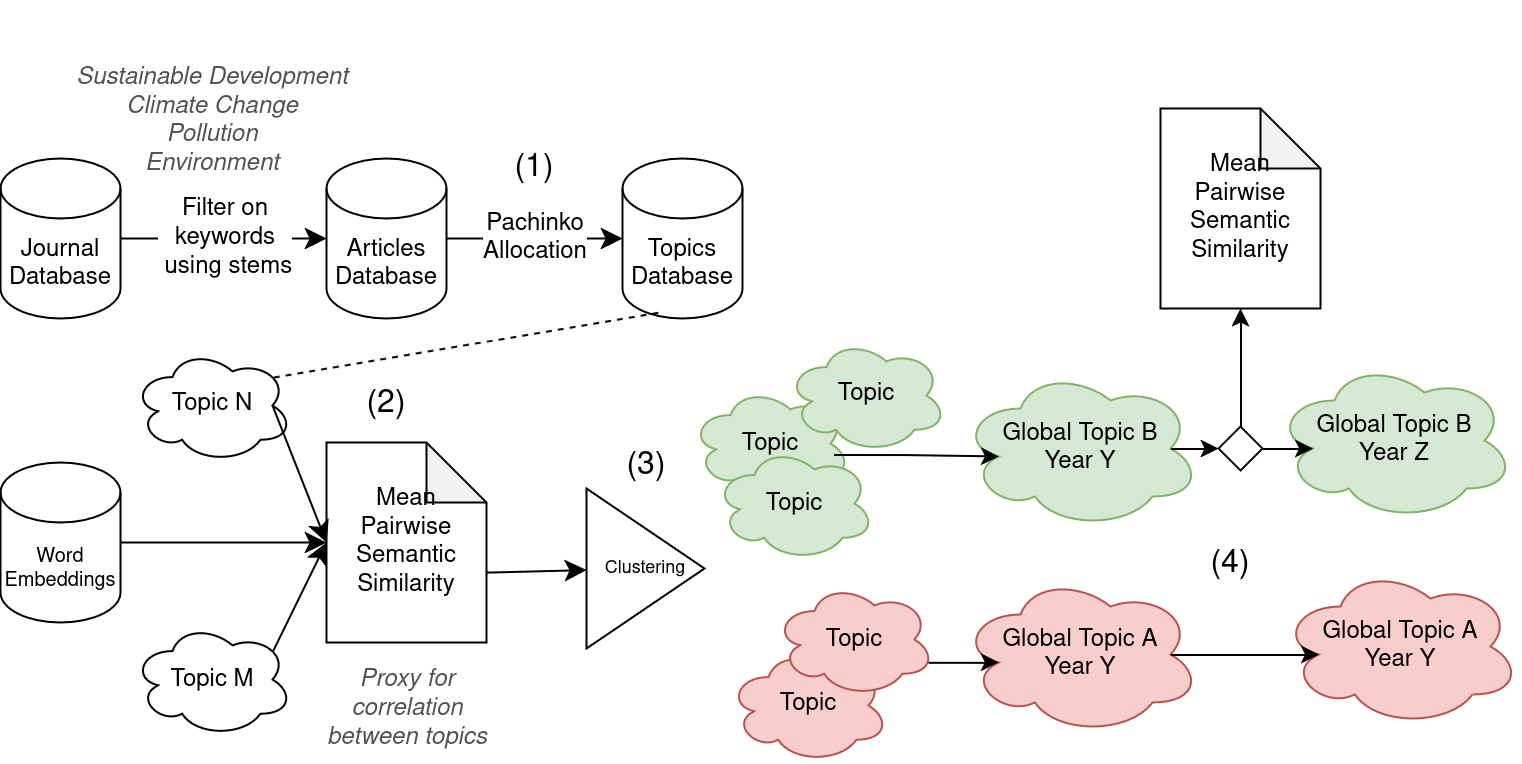
\includegraphics[width=.8\linewidth]{intro-to-ch/images/West.png}
        \caption{Description of the first 4 steps}
    \end{figure}

\end{frame}

\begin{frame}{A well observed corpus}
    Full Picture regarding Newspapers Data Availability
    \begin{itemize}
        \item Temporal coverage is explored
        \item Geographical coverage (regional newspaper vs. national) as well as political opinions explained
        \item OCR quality levels are mentioned, including the pipeline
        \item Definitions of documents 
        \begin{itemize}
            \item Document = Full Newspaper for Figaro/Imparcial
            \item Document = One Article
            \item Document = One Page
        \end{itemize}
    \end{itemize}
    With solutions for the issues for documents to "normalize" the documentary unit: using font size, capitals, etc.
\end{frame}

\begin{frame}{An adaptation of the Sustainable West paper}

    \begin{itemize}
        \item Stems + Lemmatization + Synonyms to detect keywords.
        \item Machine Translation (Google Translate) to unify representations.
        \begin{itemize}
            \item There are issues with this approach (translation could be context dependent)
            \item This is partially discussed at the keyword level (essence in France is connected to gasoline and perfume) but not at the topic model level.
        \end{itemize}
        \item Hyperparameters research explained.
    \end{itemize}
    
\end{frame}

\begin{frame}{Interesting results}

    \begin{itemize}
        \item Clear results and explanation of the results
        \item Some explanations show the limits of topic modeling approach and human labeling of topic models
        \begin{itemize}
            \item ``We additionally note mentions [of Gazoline] to the First World War in the 1910 decade, but also a report of the Franco-Prussian War in 1870 as wel as annother mention of war in 1920''. While the 1910 and 1920 are most probably tied with war and post-war issue, I have difficulties to see the connection with the F-P war. No close reading was done on this part
        \end{itemize}
    \end{itemize}
    
\end{frame}

\begin{frame}{Interesting output}
    \begin{itemize}
        \item A clear list of limitations
        \item Some close reading analysis that support or clarify some of the statements
        \item And overall, a template (computational method excluded) for such a paper: all is described, the question is clear, limitations are offered, documents and corpora are respected.
    \end{itemize}
\end{frame}

\section{Measuring a representation system}

\begin{frame}{A French / Parisien tradition}

    \begin{itemize}
        \item A. Guerreau spawned a tradition at the École nationale des Chartes and around it. Nicolas Perreaux is a direct and indirect follower of this tradition: he was the student of both Guerreau and Guerreau's former students.
        \item They use massively non-deep-learning and reproducible methods for mining information. The technological stack, at the time of the paper, did not evolve for them, despite existing new promising options. However, both the compute power and the data augmented over the course of the last 30 years. 
    \end{itemize}
    
\end{frame}

\begin{frame}{A short definition of the corpus}
    \begin{itemize}
        \item The corpus is mentioned, but this it is not described.
        \item The source of the digitization is unknown.
        \item It's quality is unknown.
        \items It's temporal coverage is unknown
    \end{itemize}
\end{frame}

\begin{frame}{A (random and not-random) topic ?}

    \begin{itemize}
        \item \textit{aqua} was chosen but it is clear from the discussion that this is partially a random choice: the question is much deeper than \textit{aqua}, and N.~Perreaux aims for a systematic (re)discovery of mundane words.
        \begin{itemize}
            \item As such, it finds it place in between Humanities focused paper and Methodology focused papers
        \end{itemize}
        \item Yet, it is describing the issue as fully as it can: how does water can be an interesting concept to question across time ?
        \item It predefines a first lexical field, including potentially disputable terms that it argues for.
    \end{itemize}
    
\end{frame}

\begin{frame}{Co-occurrence as a framework}
    \begin{itemize}
        \item Co-occurrences define relationships
        \item Study of the most frequent terms, filtering (connected 2 keywords at least)
        \item Factorial analysis
    \end{itemize}
\end{frame}

\begin{frame}{Factorial analysis ?}
    \begin{figure}
        \centering
        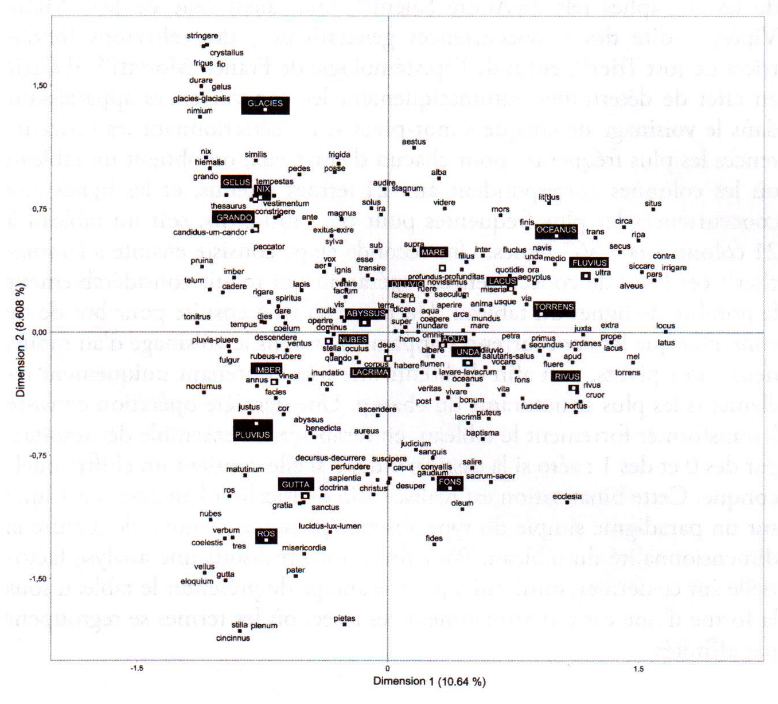
\includegraphics[width=0.5\linewidth]{intro-to-ch/images/factorial.png}
    \end{figure}
\end{frame}

\begin{frame}{Conclusions of the paper}
    \begin{itemize}
        \item It goes back to a humanities analysis at the end of the results. It's not a simple overview of the factorial analysis, but also explanations.
        \item However, it does not factor
        \begin{enumerate}
            \item Author weight: what about the sheer mass that Augustine represents in the Patrologia Latina
            \item Periods weight: this is synchronic. But Patrologia Latina = 800 years potentially.
            \item Binarization: this choice does not reflect the weight of EACH co-occurrence, and the lack of relativization of the information is detrimental to the argument.
        \end{enumerate}
    \end{itemize}
\end{frame}

\section{Conclusion}

\begin{frame}{What's the best template ?}

    \begin{enumerate}
        \item The involvement of Humanities researchers
        \item A somewhat clear question
        \item A well-defined corpus
        \item A well-defined method, even if it can be discussed
        \item A well-defined set of limitations
        \item Going back to close reading or at least bibliographic relationships
        \item Argumented and proof-based conclusions
    \end{enumerate}

    There is a strong issues with some of the papers in how they treat (1) and (2), and for some the last point. Culturomics and large scale study of texts can be a leading force in the humanities if this is done by respecting the prerequisites of the humanities (respect of the document, analysis of the biases) and of the computer sciences / statistics (well defined method, limitation analysis).
    
\end{frame}

\end{document}